\documentclass[letterpaper,11pt]{article}
\usepackage{graphicx}
\usepackage{amsmath}
\usepackage{subfig}
\usepackage{fullpage}
\usepackage{setspace}
\usepackage{ulem}

\title{Team 6 Challenge Proposal}
\author{6.141\\
	Spring 2012\\ \\
	Neil Forrester\\
	Daniel J. Gonzalez\\
	Raghavendra Srinivasan\\
	James Wiken}

\onehalfspacing				

\begin{document}
\begin{singlespacing}
\maketitle
\thispagestyle{empty}
\newpage

\tableofcontents
\listoffigures
\listoftables
\thispagestyle{empty}
\newpage

\end{singlespacing}

\setcounter{page}{1}

\section{Problem Statement}
The scenario we wish to emulate can be pictured as a robot being parachuted onto the surface of Mars with the purpose of building a shelter of some form.  Building materials have also been parachuted down and are distributed across the Martian landscape.  The robot has been provided with a map of the local area and the locations of some of the building materials.  However, some of the materials have not landed in the designated areas and thus do not show up on the map despite being useful, or perhaps essential, to the construction of the shelter.  The robot must navigate the countryside, gather materials, and use said materials to build a structure.

Similarly, our robot must perform four main tasks.  

\begin{enumerate}
 \item {\bf Navigate about an area}: The robot will be placed in a maze of some undefined size and complexity.  The robot will be provided a map of the maze beforehand and must be able to autonomously navigate the area.
 \item {\bf Locate and collect building materials}: Building materials in the form of differently colored blocks will be placed around the area.  Locations of some of the blocks will be provided with the map, but some subset of the blocks are not marked on the map.  The robot must be able to locate, recognize, and collect some subset of the blocks.
 \item {\bf Transport building materials to construction zone}: The robot must be able to move the collected blocks from their initial positions to an autonomously determined construction point.
 \item {\bf Assemble materials into a structure}: Using the collected building materials, the robot must build a structure.  The structure is roughly defined as a collection of blocks within the construction zone.  The structure can range from simple, such as a pile or a low wall, to complex, such as an enclosed room or an archway.  
\end{enumerate}

The integration of these four different abilities into a single task makes this project both interesting and challenging.  The elements needed to solve this problem can be used to further other robot applications like those listed above.  Conversely, other applications can provide at least partial solutions to this problem. 

Before proceeding with the design of a solution to the given problem statement, a series of assumptions must be made.  These assumptions can be divided into three main categories: assumptions about the environment, assumptions about the building blocks, and assumptions about the robot.

\subsection{Assumptions about the environment}
\begin{itemize}
 \item The maze is flat. While the walls stick up out of the floor, all the blocks will be sitting on the floor, and the robot will never be required to climb up or over anything, or retrieve any blocks from anywhere other than the floor.
 \item The walls of the maze are fixed, and nothing will move unless it was pushed by the robot. If the robot goes away and comes back, it can reasonably expect to find all the blocks and walls where it left them.
 \item The maze will be appropriately sized and bounded such the robot is reasonably able to explore at least the majority of the map within the the allotted challenge time. The robot also can't explore for an unlimited distance in one direction, leaving critical building materials behind.
 \item All areas of the maze will be reasonably accessible by the robot (i.e. no narrow passages, low overhangs, etc.).  All areas of the maze will be properly illuminated such that the robot can rely on vision for navigation and identification without unnecessary recalibration.
\end{itemize}
\subsection{Assumptions about the building materials}
\begin{itemize}
 \item The blocks will be reasonably sized such that the robot can easily lift them.  The block will also not be shaped such that it is incompatible with all other blocks. Ideally, the longest dimension of any block will not exceed 6 inches and all blocks will be common geometric 3D shapes.
 \item The blocks will not be unreasonably heavy such that the robot is not able to easily lift them.  The blocks will not be made of a material that is overly difficult to identify with vision (i.e. reflective surfaces, transparent/translucent, etc.).  Ideally, the blocks will be opaque plastic or painted wood.
 \item The blocks are contrasting colors from the maze walls and floor, making optical identification easier.
\end{itemize}
\subsection{Assumptions about the robot}
\begin{itemize}
 \item The base of the robot will be the same as the one we are currently using for the labs and will build on the framework built during the labs.  
 \item The battery life of the robot will be longer than the allotted time for the challenge such that is essentially a non-issue.
 \item The robot must remain within a limited budget and cannot rely on expensive sensors or manipulators to complete the challenge.
\end{itemize}

\section{High level approach and mechanical structure}
The solution we've decided on has two primary modes: collection and assembly.
In collection mode, the robot uses a funnel in front of the body to collect blocks (see figure \ref{demoFig}).
The blocks are stored in a stack under the body.
The stack is sufficiently narrow so that the blocks will interlock.
To guard against blocks getting stuck in the funnel,
there will be a break-beam sensor in the throat (not illustrated).
If a block gets stuck, the robot will back up, turn slightly, and approach the block again.

\newlength{\demowidth}
\setlength{\demowidth}{2.13in}
\newlength{\demotextwidth}
\setlength{\demotextwidth}{\demowidth}
\addtolength{\demotextwidth}{-0.15in}
\begin{figure}[h]
 \centering
  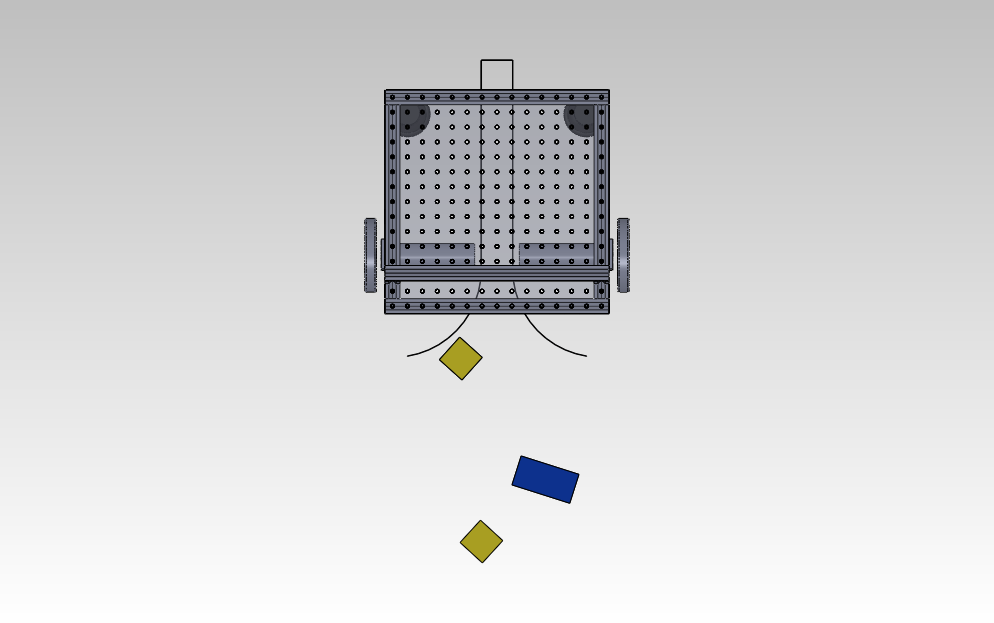
\includegraphics[width=\demowidth]{images/Demo01}
  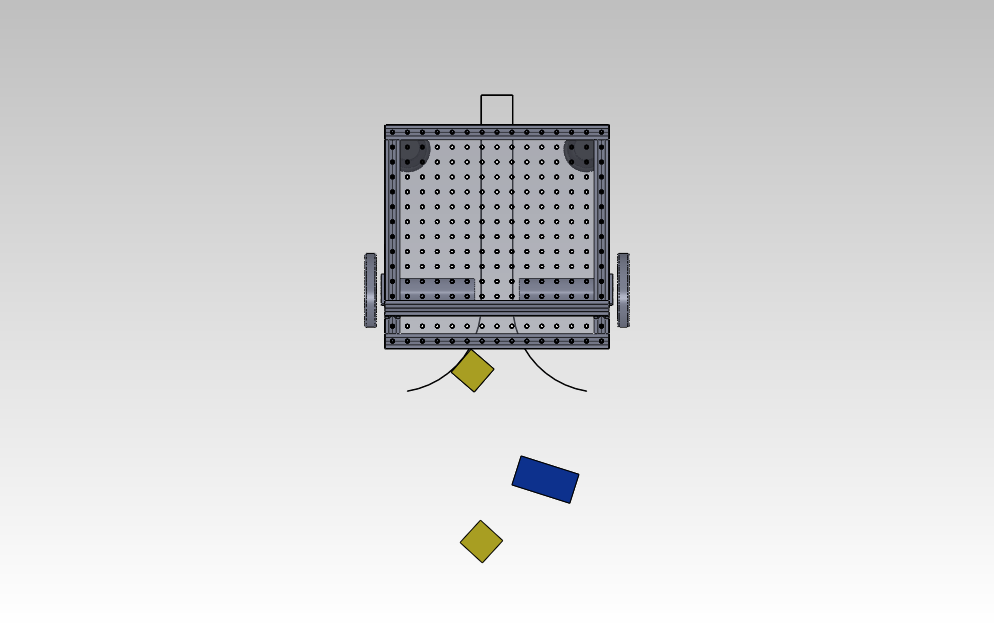
\includegraphics[width=\demowidth]{images/Demo02}
  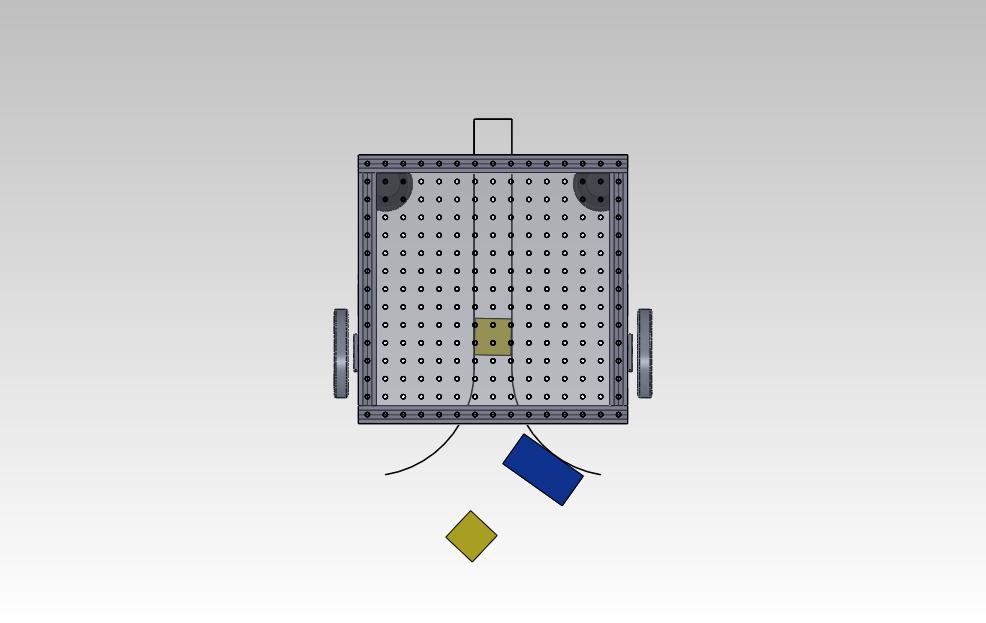
\includegraphics[width=\demowidth]{images/Demo03} \\
  1 \hspace{\demotextwidth} 2 \hspace{\demotextwidth} 3 \\
  \vspace{12pt}
  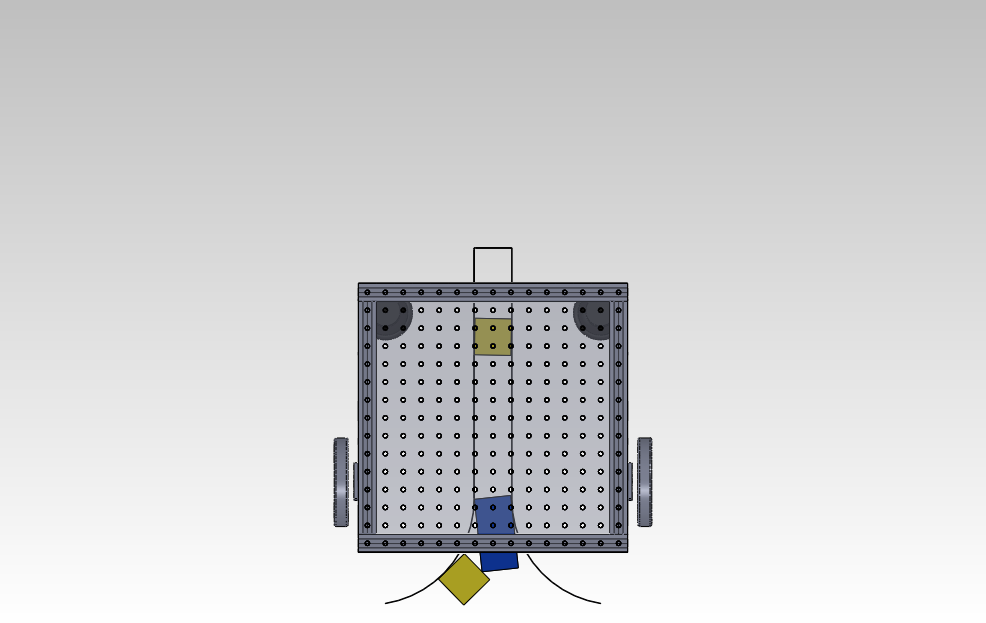
\includegraphics[width=\demowidth]{images/Demo04}
  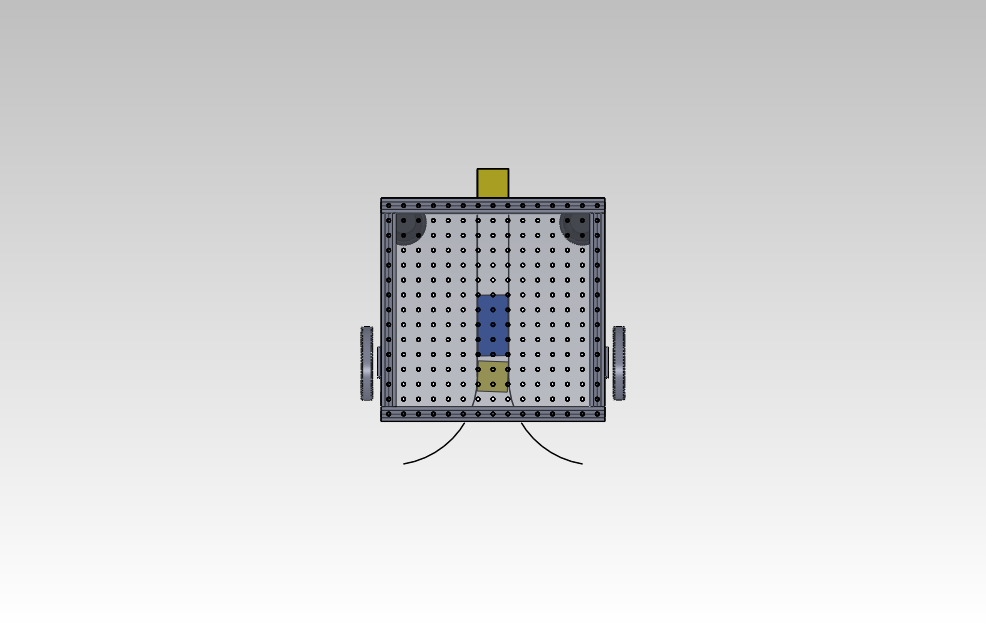
\includegraphics[width=\demowidth]{images/Demo05}
  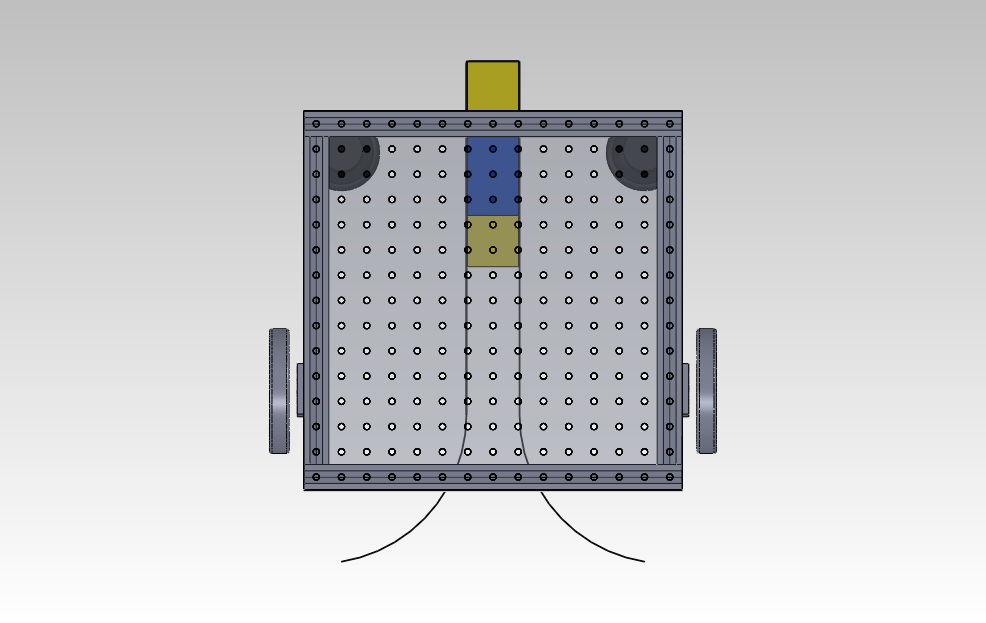
\includegraphics[width=\demowidth]{images/Demo06} \\
  4 \hspace{\demotextwidth} 5 \hspace{\demotextwidth} 6 \\
\caption{Collection Process}
\label{demoFig}
\end{figure}

After collecting a sufficient number of blocks in the stack, the robot will back up.
This will deposit the blocks in a straight line in front of the robot, and aligned with the robot center.
Now the robot will use the robotic arm to rearrange the blocks into an arbitrary planar structure.
This will be precise and efficient, because the robot will not have to turn at all to place the blocks,
and visual feedback can be used to check block placement.

\subsection{Mechanical Design}
Of the mechanical designs proposed, a system involving a simple funnel working in tandem with the manipulator built in Lab 7 was chosen.
\begin{figure}[h]
 \centering
  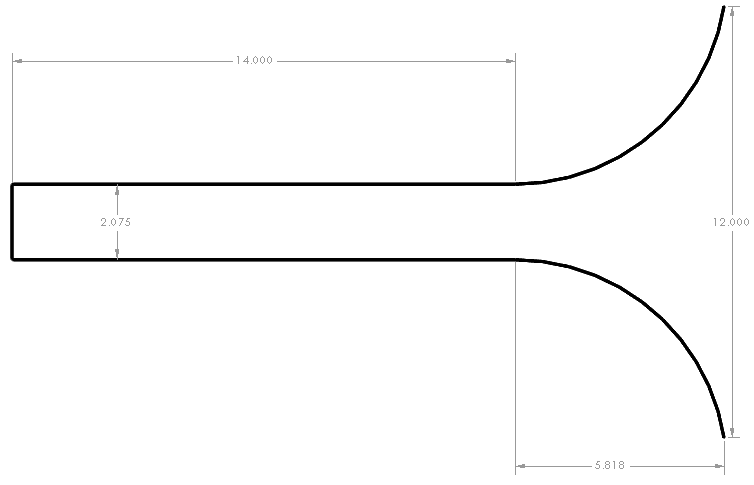
\includegraphics[width=4.5in]{images/Funnel}
\caption{Dimensioned Drawing of Funnel}
\end{figure}
\subsubsection{Funnel}
Key features include:
\begin{itemize}
\item Width of funnel is 2.075 Inches to guarantee that the blocks will "snap together" as they enter the funnel. The fillet built into each block allows a .07 Inch tolerance for "snapping "
\item The funnel will be placed in the center to minimize the robot's footprint and account for errors in visual servoing. The surfaces are gently curved to guide the blocks into the funnel.
\item Long funnel Increasing the length of the funnel would increase our robot's block storage capacity but inhibit its mobility by increasing its footprint.
\item asdasdasd
\end{itemize}
Solidworks simulations proved 

\subsubsection{Manipulator}


\section{Systems}
%TODO: do we want any text here?b
\begin{figure}[h]
\centering
 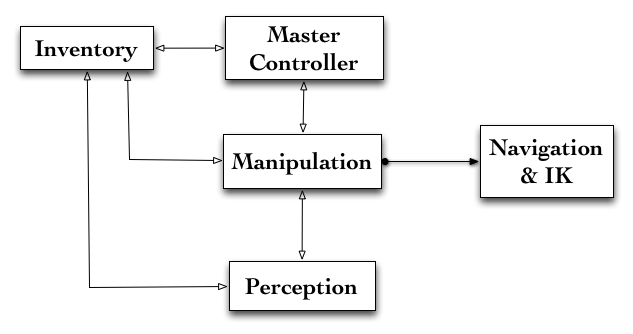
\includegraphics[width=4in]{images/System_Architecture}
\caption{System Architecture}
\end{figure}

\subsection{Master Controller}
The Master Controller is the brain of the system, does high-level planning, and decides when to stop.
High level operations will be broken down and handed out to other modules for execution.
%TODO: do we want to say anything more about this?

\subsection{Inventory and Mapping}
The Inventory and Mapping module provides the other modules with information about the environment.
This information includes the poses of blocks in the environment,
the blocks in the stack under the robot,
the walls of the maze,
the robot's current location,
and anything else we decide is useful.
The I\&M module takes input from the Perception module, and performs data fusion, mapping, and localization.
%TODO: do we want to say anything more about this?

\subsection{Navigation and Inverse Kinematics}
The Navigation and Inverse Kinematics module directly controls the robot's actuators.
Other modules give it commands such as ``travel to $(x, y, \theta)$'',
or ``Move the robotic arm gripper to $(x, y, z, \theta, \phi)$'',
and the N\&IK module will move the robot appropriately.
%TODO: do we want to say anything more about this?

\subsection{Manipulator}
The Manipulator takes commands from the Master Controller
and decides what motions need to be performed to manipulate the blocks.
For example, if the Master Controller commands ``collect block 42'',
the Manipulator will order the N\&IK module to make movements that will funnel the block into the stack.
%TODO: do we want to say anything more about this?

\subsection{Perception}
The Perception module reads data from the sensors and feeds information to the Inventory and Mapping module.
For example, if the camera image contains a hexagonal red blob,
the Perception module will interpret this as a block at an angle,
and report the presence of a block to the I\&M module.
%TODO: do we want to say anything more about this?

\section{Schedule}
\begin{tabular}{r | l}
Task & Timeframe\\
\hline
\sout{Steal} Obtain materials    & today \\
Build the funnel                 & tomorrow \\
Write code to collect blocks     & The Day After Tomorrow \\
Write code to assemble structure & 1984
\end{tabular}
%TODO: text here

\section{Conclusion}
The design described above fulfills the requirements as set by the problem statement. The robot will be able to navigate the environment, identify and collect blocks, transport them to a construction zone, and fabricate a structure. This design prioritizes speed of block collection through the use of a center-mounted funnel as a simple collection device. This allows for the extra time a more complex construction method requires, such as the motion planning approach used by the robot's arm. This approach allows the structure design to be generalized as many different structures can be built in this manner. However, this method leaves room for error as the motion planning will likely be open loop which may cause an archway to quickly become a pile (which is still a structure). Despite these caveats, the design detailed above is a promising solution to the grand challenge for 6.141.
\end{document}
